\documentclass[conference]{IEEEtran}
\IEEEoverridecommandlockouts

\usepackage{cite}
\usepackage{amsmath,amssymb,amsfonts}
\usepackage{algorithmic}
\usepackage{graphicx}
\usepackage{textcomp}
\usepackage{xcolor}
\usepackage{booktabs}
\usepackage{array}
\usepackage{multirow}
\usepackage{url}
\usepackage{hyperref}
\usepackage{balance}

\hypersetup{colorlinks=true, linkcolor=blue, citecolor=blue, urlcolor=blue}

\def\BibTeX{{\rm B\kern-.05em{\sc i\kern-.025em b}\kern-.08em
    T\kern-.1667em\lower.7ex\hbox{E}\kern-.125emX}}

% figures live in exports/figures/ ; adjust or copy alongside this .tex
\graphicspath{{./}}

\begin{document}

\title{Parallel Consensus Routing: Training-Free Quality Control, Coordinated
Hallucination, and Model-Pair Selection in Cost-Efficient LLM Inference}

\author{
\IEEEauthorblockN{Aksh Modi}
\IEEEauthorblockA{
\textit{Independent AI Research}\\
Manipal University Jaipur, Rajasthan, India
}
}

\maketitle

\begin{abstract}
Cost-efficient large language model (LLM) inference is dominated by two
paradigms: \textit{pre-query routing}, which commits to a model before any
output exists, and \textit{sequential cascading}, which escalates cheap-to-expensive
in series and accrues additive latency. We study \textbf{Parallel Consensus
Routing (PCR)}, a third paradigm that runs two inexpensive models simultaneously
and uses their binary output agreement as a training-free quality oracle: agreed
queries are resolved immediately, disagreements trigger exactly one frontier
escalation. We run a \textbf{balanced four-pair design} --- two within-family and
two cross-family cheap pairs, with the frontier model and the serving provider
held constant --- on a \textbf{complete six-benchmark grid} (ARC, OpenBookQA,
CommonsenseQA, MMLU, TruthfulQA, MMLU-Pro), all 24 cells populated, scoring
\textbf{eight routing policies} on identical stored data. Every pair reported
completed all six benchmarks; pairs that finished only a subset were excluded
rather than shown with gaps. Five results emerge. (1) \textbf{Coordinated
hallucination (C-Hall)}---two cheap models agreeing on a wrong answer---%
\textbf{scales monotonically with question difficulty, not task type}: the mean
rises from $\approx$3\% on ARC/OpenBookQA to $\approx$19\% on MMLU-Pro (25.9\%
for the within-family Qwen pair), reaching on a plain multiple-choice task the
error rates previously reported only for mathematical reasoning.
(2) A \textbf{capability-matched} cheap pair with PCR matches always-frontier
accuracy on easy/medium questions at 40--70\% lower cost, but on hard questions
its accuracy is safe while its C-Hall (12--26\%) is not. (3) \textbf{Shared model
lineage} buys a large agreement premium on hard/adversarial benchmarks
($+9$ to $+22$\,pp; CommonsenseQA, TruthfulQA, MMLU-Pro) and, suggestively, a
coordinated-hallucination premium there too (TruthfulQA $+6.6$\,pp, CI
$[+0.3,+12.8]$); on easy/medium benchmarks neither effect appears. With two pairs
per condition the C-Hall signal is a hypothesis for powered follow-up. What makes
a pair usable at all is capability matching, not lineage. (4) A \textbf{third cheap model}
(PCR-3, majority vote) reliably breaks ties but yields no accuracy or safety
gain. (5) On free-tier APIs, \textbf{two of \{gpt-oss-20B, Qwen3.6-27B,
Qwen3.8-27B\} on a low-latency provider} is the recommended default: solo
accuracies within $\sim$1\,pp, $\approx$0.5\,s latency, $\approx$5--12\%
escalation. All experiments used free-tier inference and required \$0 marginal
API spend.
\end{abstract}

\begin{IEEEkeywords}
LLM routing, cost-efficient inference, parallel consensus, coordinated
hallucination, model-pair selection, capability matching, black-box API inference
\end{IEEEkeywords}

%===========================================================
\section{Introduction}
%===========================================================

The LLM API marketplace is sharply tiered: frontier models command costs one to
two orders of magnitude above small open models \cite{bommasani2021}. For
throughput workloads, routing \textit{all} queries to a frontier is
prohibitively expensive and routing all to a cheap model forfeits quality on the
hard tail. The engineering problem is: \textit{given a query, which model or
combination minimizes cost subject to a quality constraint?}

Three paradigms exist. \textbf{Pre-query routing}
\cite{ong2024routellm,ding2024hybrid} predicts the right tier from input
features before any output is generated. \textbf{Sequential cascading}
\cite{chen2023frugalgpt} queries cheap first and applies a learned scorer to
decide escalation, adding one model's latency per hop.
\textbf{Self-verification routing} \cite{aggarwal2024automix} lets a small model
grade its own answer, but self-verification is noisy on reasoning
\cite{kadavath2022}.

We study a structurally different idea: \textbf{use two cheap models as quality
oracles for each other}. Two independently deployed cheap models queried in
parallel that converge on the same answer provide agreement evidence that is
stronger than either model's self-assessment. On disagreement, exactly one
frontier call is made. The system is training-free, black-box compatible, and
faster than a serial cascade on every agreed query. The analogy to speculative
decoding \cite{leviathan2023,chen2023speculative} is exact---draft-then-verify
at the response level rather than the token level---but without the white-box
probability access speculative decoding requires.

The failure mode that makes this non-trivial is \textbf{coordinated
hallucination (C-Hall)}: two cheap models agreeing on the \textit{same wrong}
answer. C-Hall is invisible to the router---it is indistinguishable from correct
consensus---so understanding when it occurs is a safety prerequisite, not an
optimization.

\paragraph{Contributions} This paper (i) reproduces and extends an initial
single-pair PCR study with a \textbf{balanced 4-pair design on a complete
6-benchmark grid} (frontier and provider held constant), every cell populated; (ii) shows C-Hall \textbf{scales with difficulty, not task type},
generalizing the earlier ``knowledge vs.\ math'' dichotomy to a difficulty-tier
one; (iii) runs a \textbf{full 8-policy ablation} (Always-Cheap, Best-Cheap,
Consensus, PCR-2, Oracle-2-cheap, Random, Always-Frontier, PCR-3) on identical
data; (iv) characterizes the \textbf{model-family effect}---a large agreement
premium and a suggestive coordinated-hallucination premium, both on
hard/adversarial benchmarks only---and identifies \textbf{capability matching} as
the constraint that makes a pair usable at all; (v) provides measured
cost/latency and a concrete
\textbf{practitioner pair-selection guide}.

%===========================================================
\section{Related Work}
%===========================================================

\subsection{Sequential Cascade Routing}
FrugalGPT \cite{chen2023frugalgpt} defines an LLM cascade with a learned
(DistilBERT) accept/escalate scorer, matching GPT-4 at up to 98\% cost reduction
on classification, but requiring task-specific supervised training and incurring
latency proportional to cascade depth. Hybrid LLM \cite{ding2024hybrid} predicts
the small-vs-large quality gap pre-query (up to 40\% fewer large calls,
$<$1\% quality drop) but cannot use observed output. AutoMix
\cite{aggarwal2024automix} is architecturally closest to PCR: a single model
self-verifies before escalation, with a POMDP meta-verifier absorbing
self-verification noise. Our cross-model agreement is stronger than
self-verification in principle---independent models cannot share a
self-delusion---though, as our matrix shows, shared training corpora still
induce correlated errors.

\subsection{Pre-Query Routing}
RouteLLM \cite{ong2024routellm} trains four router variants on Chatbot Arena
preference data ($>$85\% cost reduction on MT-Bench, 45\% on MMLU). GraphRouter
\cite{feng2024graphrouter} models query--LLM relationships with GNNs; FORC
\cite{sakota2024forc} learns per-LLM score prediction via contrastive learning;
RouterBench \cite{hu2024routerbench} standardizes evaluation. All require trained
components; PCR requires none.

\subsection{Multi-Model Consensus and Ensembles}
Multi-agent debate \cite{du2023multiagent} improves reasoning through iterative
text exchange at $O(\text{rounds}\times\text{models})$ cost. Self-Consistency
\cite{wang2023selfconsistency} majority-votes multiple samples from one model;
LLM-Blender \cite{jiang2023llmblender} fuses open-model outputs with a trained
ranker; ChatEval \cite{chan2023chateval} debates for evaluation. None exploit
cost differentials between tiers, and none use a single-round binary agreement
signal.

\subsection{Speculative Decoding}
Leviathan et al.\ \cite{leviathan2023} and Chen et al.\
\cite{chen2023speculative} accelerate decoding with a draft model whose tokens
the target verifies by rejection sampling (2--3$\times$ speedup, provable
equivalence). This needs the target's per-token distribution---unavailable for
proprietary APIs. PCR realizes the same draft-then-verify separation at the
\textit{response} level on final text only.

\subsection{Semantic Caching, Calibration, and Hallucination}
vCache \cite{schroeder2025vcache} shows global similarity thresholds carry no
correctness guarantee and proposes per-embedding online learning; our
per-domain/per-difficulty threshold table is the routing analogue.
SelfCheckGPT \cite{manakul2023selfcheckgpt} detects hallucination via
multi-sample consistency; Kadavath et al.\ \cite{kadavath2022} show LLMs are
poorly calibrated on multi-step reasoning. Coordinated hallucination---agreement
\textit{negatively} correlated with correctness on hard items---has not been
characterized in the routing literature.

\subsection{Benchmarks}
Our grid spans MMLU \cite{hendrycks2020mmlu} and ARC-Challenge
\cite{clark2018arc}, plus TruthfulQA \cite{lin2022truthfulqa} (adversarial
misconceptions), MMLU-Pro \cite{wang2024mmlupro} (10-option, reasoning-heavy),
OpenBookQA \cite{mihaylov2018openbookqa} and CommonsenseQA \cite{talmor2019csqa}
--- six multiple-choice sets that span a wide difficulty range while holding the
answer format fixed. We exclude numeric-answer benchmarks such as GSM8K
\cite{cobbe2021gsm8k} from the grid: there, answer extraction interacts with the
generation budget, which confounds the agreement measurement
(\S\ref{sec:futurework}). Chain-of-thought \cite{wei2022cot} is suppressed to
isolate the agreement signal.

\begin{table*}[!t]
\caption{Literature Review --- Related Work and Differentiation of Contribution}
\label{tab:litreview}
\renewcommand{\arraystretch}{1.2}
\begin{tabular}{p{2.6cm} p{1.9cm} p{3.2cm} p{3.4cm} p{3.6cm}}
\toprule
\textbf{Reference} & \textbf{Year/Venue} & \textbf{Approach} & \textbf{Key Limitation} & \textbf{PCR Advantage} \\
\midrule
FrugalGPT \cite{chen2023frugalgpt} & 2023 / TMLR & Sequential cascade, trained quality scorer & Labeled training data; serial latency & Training-free; parallel; bounded at one frontier call \\
Hybrid LLM \cite{ding2024hybrid} & 2024 / ICLR & Pre-query difficulty-gap router & No output signal; pre-commit & Post-query observed agreement \\
RouteLLM \cite{ong2024routellm} & 2024 / arXiv & Preference-trained router (4 variants) & Human preference labels & Zero labeled data; any API pair \\
AutoMix \cite{aggarwal2024automix} & 2024 / ACL & Self-verify + POMDP router & Self-verification noisy; POMDP training & Cross-model verification; training-free \\
Multi-agent Debate \cite{du2023multiagent} & 2024 / ICML & Iterative multi-round debate & $O(\text{rounds}\times\text{models})$; high latency & Single-round; throughput-optimized \\
Self-Consistency \cite{wang2023selfconsistency} & 2023 / ICLR & Majority vote, one model & Same tier; no cost cut & Cross-tier; cheap replaces expensive samples \\
Spec.\ Decoding \cite{leviathan2023,chen2023speculative} & 2023 / ICML & Draft-then-verify on token probs & White-box only & Black-box; final text only \\
vCache \cite{schroeder2025vcache} & 2025 / arXiv & Online per-embedding threshold & Caching, not routing & Per-domain/difficulty calibration for routing \\
SelfCheckGPT \cite{manakul2023selfcheckgpt} & 2023 / EMNLP & Multi-sample consistency & Consistency assumed positive & C-Hall: consistency as \emph{negative} indicator on hard items \\
RouterBench \cite{hu2024routerbench} & 2024 / arXiv & Routing benchmark & No algorithm proposed & Results compatible with its methodology \\
\bottomrule
\end{tabular}
\end{table*}

\subsection{Research Gap}
No prior work evaluates a \textit{parallel binary-consensus} quality oracle for
cost reduction, characterizes coordinated hallucination and its
difficulty-dependence, controls for model-family relatedness while holding
capability constant, or provides an empirical pair-selection guide for
practitioners. This paper does all four.

%===========================================================
\section{Methodology}
%===========================================================

\subsection{Problem Formulation}
Let $M_A, M_B$ be cheap models and $M_F$ a frontier model, with
$\text{cost}(M_F)\gg\text{cost}(M_A)\approx\text{cost}(M_B)$. For a
multiple-choice query $q$ each model emits a letter $r\in\{$A$,\dots\}$. The
\textbf{PCR-2} decision rule is
\begin{equation}
\text{output}(q)=\begin{cases}
r_A(q) & r_A(q)=r_B(q)\quad\text{[agreement]}\\
M_F(q) & r_A(q)\neq r_B(q)\quad\text{[disagreement]}
\end{cases}
\end{equation}
with expected per-query cost
$\mathbb{E}[\text{cost}]=\text{cost}(M_A)+\text{cost}(M_B)+\text{cost}(M_F)\cdot P(\text{disagree})$.

\subsection{PCR-3: Majority Vote}
\textbf{PCR-3} runs three cheap models $M_A,M_B,M_C$; if any two agree, their
answer is taken; only if all three differ is $M_F$ called. This trades one
extra cheap call for a lower escalation rate and a majority-vote margin.

\subsection{Policy Space}
Every policy below is scored on the \textit{same} stored per-question data
(cheap answers, agreement, frontier answer on disagreements, per-call token and
latency instrumentation), so no policy requires additional API calls except
Always-Frontier (see \S\ref{sec:setup}):
\emph{Always-Cheap-A/-B} (one small model);
\emph{Best-Cheap} (the stronger of the two);
\emph{Consensus, no escalation} (trust agreement, fall back to $M_A$ on
disagreement---provably equal to Always-Cheap-A);
\emph{PCR-2}; \emph{Oracle-2-cheap} (correct whenever \textit{either} cheap
model is correct---the ceiling for any two-cheap method);
\emph{Random} (coin flip $M_A$ vs.\ $M_F$);
\emph{Always-Frontier}; \emph{PCR-3}.

\subsection{Agreement Signal and Outcome Categories}
We optionally compute embedding cosine similarity $s\in[-1,1]$ between raw
responses (\texttt{all-MiniLM-L6-v2} \cite{reimers2019sentencebert}). Three
outcome categories: \textbf{correct consensus} ($r_A=r_B=$ gold);
\textbf{coordinated hallucination} ($r_A=r_B\neq$ gold);
\textbf{disagreement} ($r_A\neq r_B$).

\subsection{Coordinated Hallucination Hypothesis}
We hypothesize C-Hall arises from shared inductive biases in overlapping
training corpora: on retrieval both models recall the same fact (beneficial),
on procedural or adversarial items both may pattern-match the same wrong
shortcut or misconception. We test two moderators: (a) benchmark
\textbf{difficulty}, and (b) whether the pair is \textbf{within-family} (same
developer/lineage) or \textbf{cross-family}.

\subsection{Capability Matching}
A within-vs-cross comparison is only interpretable if the two cheap models are
capability-matched: if one model is much weaker, high agreement reflects the
weak model deferring to a shared plausible-wrong answer (a skill gap), not
family structure. We require the two cheap models' \textit{solo} accuracy to
differ by $\leq 3$\,pp on each benchmark; cells violating this are reported but
excluded from family pooling.

\subsection{Difficulty Tiers}
We group the six benchmarks by observed difficulty: \textbf{easy}
(ARC-Challenge, OpenBookQA, CommonsenseQA), \textbf{medium} (MMLU), and
\textbf{hard} (TruthfulQA, MMLU-Pro).

%===========================================================
\section{Experimental Setup}
\label{sec:setup}
%===========================================================

\subsection{Inclusion criterion}
\label{sec:inclusion}
Every result in this paper comes from a pair that completed \textbf{all six
benchmarks at full $N$}. We screened eleven candidate pairs; seven were dropped
before analysis --- two used models the providers delisted mid-study, two ran on
only one or two benchmarks, and three were blocked partway by a provider's
free-tier cap (two of those also failed the capability-matching bar of
\S\ref{sec:capmatch}). Reporting a pair on a subset of benchmarks would make
cross-pair comparison depend on which cells happened to finish, so those pairs
are excluded entirely rather than shown with gaps. What remains is a
\textbf{balanced $4\times6$ design}: two within-family pairs and two
cross-family pairs, all sharing one frontier model and one provider
(Table~\ref{tab:pairs}), with 24 of 24 cells populated.

\subsection{Models}
All models are free tier. Cheap models: \texttt{gpt-oss-20b},
\texttt{gpt-oss-safeguard-20b} (both OpenAI-oss), \texttt{qwen3.6-27b},
\texttt{qwen3.8-27b} (both Alibaba Qwen3) --- all $\leq$27B and served on Groq.
Frontier: \texttt{gpt-oss-120b}, identical for all four pairs, so frontier
capability is held constant and only the cheap-pair lineage varies.

\subsection{Benchmarks}
Six multiple-choice benchmarks (Table~\ref{tab:benchmarks}), spanning
elementary science to adversarial misconceptions and 10-option reasoning. Letter
extraction is generalized to A--J. TruthfulQA MC1 is reduced to 6 options (the
true option plus $\leq 5$ sampled distractors, shuffled per question) for
comparability. Cheap answer budget is 256 tokens throughout (measured:
reasoning-tuned cheap models need $\sim$200 hidden tokens before emitting a
letter). We deliberately restrict to a single answer format: a numeric-answer
benchmark was piloted but is excluded, because answer extraction there is
confounded with the token budget (\S\ref{sec:futurework}).

\begin{table}[!t]
\caption{Benchmarks. Every pair in this study is evaluated on all six.}
\label{tab:benchmarks}
\renewcommand{\arraystretch}{1.15}
\begin{tabular}{p{2.3cm} c p{1.0cm} p{2.6cm}}
\toprule
\textbf{Benchmark} & \textbf{Options} & \textbf{$N$} & \textbf{Character} \\
\midrule
OpenBookQA & A--D & 200 & elementary science \\
ARC-Challenge & A--E & 150--300 & science reasoning \\
CommonsenseQA & A--E & 200 & commonsense \\
MMLU & A--D & 250 & general knowledge, 57 domains \\
TruthfulQA (MC1) & A--F & 150 & adversarial misconceptions \\
MMLU-Pro & A--J & 150 & hard, reasoning-heavy \\
\bottomrule
\end{tabular}
\end{table}

\subsection{Model pairs}
The four pairs meeting the inclusion criterion (Table~\ref{tab:pairs}) form a
$2\times2$ design: lineage (within-family vs.\ cross-family) crossed with two
distinct model choices per condition. All four share the frontier
(\texttt{gpt-oss-120b}) and the provider, so neither confounds the comparison.
Pairs~10--11 were constructed after the solo sweep (below) identified
\texttt{gpt-oss-20b}, \texttt{qwen3.6-27b} and \texttt{qwen3.8-27b} as mutually
capability-matched to $\sim$1\,pp. A three-model trio drawn from the same set is
used for the PCR-3 ablation.

\begin{table}[!t]
\caption{The four pairs. Family = whether the two cheap models share a
developer/lineage. Frontier and provider are constant across all four.}
\label{tab:pairs}
\renewcommand{\arraystretch}{1.25}
\footnotesize
\setlength{\tabcolsep}{4pt}
\begin{tabular}{l l l l}
\toprule
\textbf{Pair} & \textbf{Family} & \textbf{Cheap A} & \textbf{Cheap B} \\
\midrule
Pair 3 & within & gpt-oss-20b & gpt-oss-safeguard-20b \\
Pair 7 & within & qwen3.8-27b & qwen3.6-27b \\
Pair 10 & cross & gpt-oss-20b & qwen3.6-27b \\
Pair 11 & cross & gpt-oss-20b & qwen3.8-27b \\
\midrule
PCR-3 trio & --- & \multicolumn{2}{l}{gpt-oss-20b + qwen3.6-27b + qwen3.8-27b} \\
\bottomrule
\multicolumn{4}{p{8.4cm}}{\footnotesize Frontier for every row: \texttt{gpt-oss-120b}. Provider for every row: Groq.}
\end{tabular}
\end{table}

\subsection{Solo model sweep and capability gaps}
Each model was run \textit{alone} ($N=80$/benchmark) to measure standalone
accuracy (Table~\ref{tab:solo}, upper block). This provides the Always-Frontier
baseline used throughout the ablation, and lets each pair's capability gap be
read directly (lower block).

Three of the four benchmarks put every pair inside the $\pm3$\,pp matching bar of
\S\ref{sec:capmatch}. \textbf{TruthfulQA is the exception}: \texttt{gpt-oss-20b}
is markedly weaker there (71.2) than either Qwen model (81.2/83.8), so the two
\textit{cross}-family pairs carry 10.0 and 12.6\,pp gaps on that benchmark while
the within-family pairs stay at 2.6--3.8\,pp. We report this rather than drop the
cells, because the confound runs \textit{against} our main family result: a
mismatched pair should show \textit{inflated} C-Hall (\S\ref{sec:capmatch}), yet
on TruthfulQA the mismatched cross-family pairs show the \textit{lower} C-Hall
(9.5\%, 11.2\%) and the matched within-family pairs the higher (14.3\%, 19.8\%).
The within-family premium of Finding~5 therefore survives a bias pointed the
opposite way; it is not an artifact of mismatch.

\begin{table}[!t]
\caption{\textbf{Upper:} solo accuracy of every model in this study ($N=80$).
\textbf{Lower:} the resulting per-pair capability gap $|$Cheap\,A $-$ Cheap\,B$|$
in pp. Bold = exceeds the $\pm3$\,pp matching bar.}
\label{tab:solo}
\renewcommand{\arraystretch}{1.15}
\begin{tabular}{l c c c c}
\toprule
\textbf{Model} & \textbf{ARC} & \textbf{MMLU} & \textbf{M-Pro} & \textbf{TQA} \\
\midrule
gpt-oss-120b \textit{(frontier)} & 95.0 & 82.5 & 71.2 & 78.8 \\
\midrule
gpt-oss-20b & 96.2 & 82.5 & 65.0 & 71.2 \\
gpt-oss-safeguard-20b & 93.8 & 85.0 & 63.7 & 75.0 \\
qwen3.6-27b & 96.2 & 82.5 & 63.7 & 81.2 \\
qwen3.8-27b & 95.0 & 86.2 & 63.7 & 83.8 \\
\midrule
\multicolumn{5}{c}{\textit{Per-pair capability gap (pp)}} \\
\midrule
Pair 3 (within) & 2.4 & 2.5 & 1.3 & 3.8 \\
Pair 7 (within) & 1.2 & 3.7 & 0.0 & 2.6 \\
Pair 10 (cross) & 0.0 & 0.0 & 1.3 & \textbf{10.0} \\
Pair 11 (cross) & 1.2 & 3.7 & 1.3 & \textbf{12.6} \\
\bottomrule
\multicolumn{5}{p{8.4cm}}{\footnotesize OpenBookQA and CommonsenseQA were not part of the solo sweep; pair-level capability there is visible in the easy-tier Best-Cheap column of Table~\ref{tab:policytier}, where the four pairs span 88.6--93.8\%.}
\end{tabular}
\end{table}

\subsection{Infrastructure}
Python 3.13, \texttt{asyncio} for parallel cheap calls, temperature 0, seed 42,
no chain-of-thought. A checkpoint-and-resume mechanism (every 50 questions, plus
a crash-safety flush) tolerates rate-limit interruptions; a cap-aware job queue
defers rate-limited work and resumes it after daily resets. Per-call token and
wall-clock latency are recorded for cost/latency analysis. All runs used
free-tier APIs; total marginal API spend \$0.

\subsection{Ablation design}
All policy-ablation rows for a given (pair, benchmark) share one stored result
set; only the decision rule differs. Always-Frontier accuracy is taken from the
solo sweep (Table~\ref{tab:solo}). PCR-3 is run separately ($N=120$/benchmark).

%===========================================================
\section{Results and Discussion}
\label{sec:results}
%===========================================================

\subsection{Finding 1: C-Hall scales with difficulty, not task type}
Prior work characterises coordinated hallucination as a \textit{task-type} split
--- low on knowledge retrieval ($\approx$9\%), high on mathematical reasoning
($\approx$32\%) --- and prescribes task-type routing accordingly. On the
consistent 4-pair grid the effect is instead a smooth monotone climb with
question difficulty, entirely \textit{within} knowledge tasks
(Table~\ref{tab:ladder}, Fig.~\ref{fig:ladder}): the mean agreed-answer error
rate rises from $\approx$3\% on ARC/OpenBookQA to $\approx$19\% on MMLU-Pro, and
for the within-family Qwen pair (Pair~7) reaches \textbf{25.9\% on MMLU-Pro} ---
the error rate previously attributed to mathematical reasoning, here on a
256-token multiple-choice task with $<$3\% unparsed responses. It is a property
of question difficulty, not of the answer format or the task type.

\begin{table}[!t]
\caption{C-Hall rate on agreed questions, by benchmark (mean over the 4 complete
pairs; range across pairs in parentheses).}
\label{tab:ladder}
\renewcommand{\arraystretch}{1.15}
\begin{tabular}{l c l}
\toprule
\textbf{Benchmark} & \textbf{Mean C-Hall} & \textbf{Tier} \\
\midrule
OpenBookQA & 3\% \;(1.6--4.5) & easy \\
ARC-Challenge & 3\% \;(2.6--3.9) & easy \\
MMLU & 10\% \;(8.3--11.3) & medium \\
CommonsenseQA & 10\% \;(7.1--15.6) & easy \\
TruthfulQA & 14\% \;(9.5--19.8) & hard \\
MMLU-Pro & 19\% \;(13.3--25.9) & hard \\
\bottomrule
\end{tabular}
\end{table}

\begin{figure}[!t]
\centering
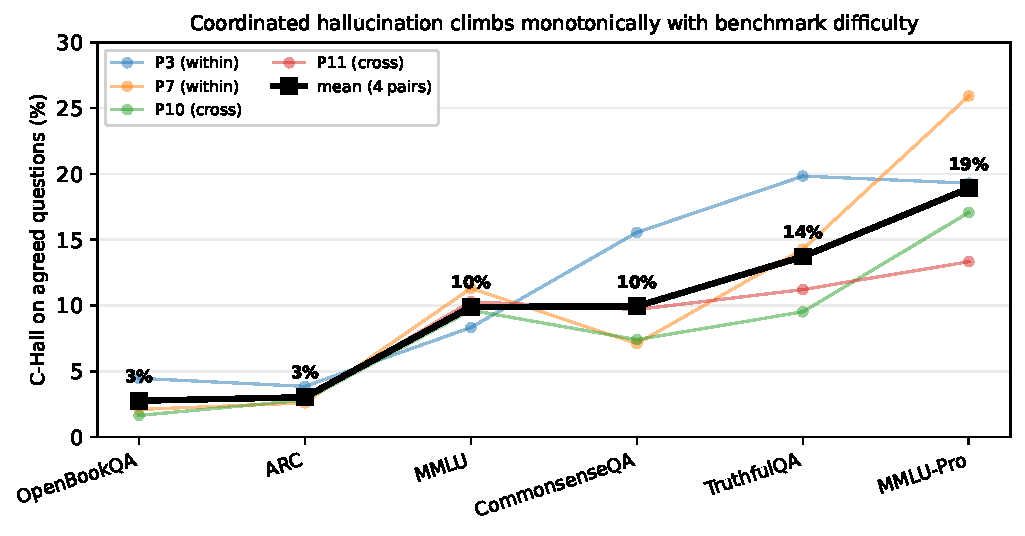
\includegraphics[width=\columnwidth]{fig_chall_ladder}
\caption{Coordinated hallucination across the four pairs, all six benchmarks.
The mean climbs monotonically with difficulty ($\approx$3\% $\to$ 19\%); the
within-family Qwen pair (P7) reaches 25.9\% on MMLU-Pro --- an error rate
previously reported only for mathematical reasoning, here on a plain
multiple-choice task.}
\label{fig:ladder}
\end{figure}

\textbf{The prerequisite for safe PCR is difficulty-tier awareness, not
task-type awareness.} A trust threshold should be calibrated on question
difficulty, which the escalation rate itself estimates (\S
ef{sec:earns}).
CommonsenseQA is the one non-monotone point ($\approx$10\%,
between MMLU and the easy pair): its C-Hall is driven by Pair~3, whose
safety-tuned model produces 15.6\% there.

\subsection{Finding 2: Full policy ablation}
Table~\ref{tab:policytier} scores eight policies by difficulty tier.
\textbf{Easy:} on ARC every pair is within $\approx$1\,pp of Always-Frontier
(95.0\%) and PCR-2's only value is cost; CommonsenseQA is
harder than its ``easy'' label suggests (C-Hall 7--16\%), which is why the
per-pair easy-tier means span 89--93\%. \textbf{Medium:} PCR-2 adds +1 to
+16\,pp over Best-Cheap depending on cheap-model strength, and the two all-Groq
cross-family pairs (10, 11) reach 86--88\% --- above Always-Frontier's 82.5\%.
\textbf{Hard:} all four pairs land at 76.7--78.3\% ---
\textit{matching or beating} Always-Frontier (75.0\%). But 12--20\% of the
answers PCR-2 trusts on the hard tier are wrong, so the accuracy is real and the
safety is not; the within-family pairs (3, 7) carry the higher C-Hall (20\%)
versus the cross-family pairs (12--13\%), consistent with Finding~5.
\textbf{Oracle-2-cheap} (right if either cheap model is right) sits 3--5\,pp
above PCR-2 on several cells --- a smarter-than-binary selector has real
headroom.

\begin{table}[!t]
\caption{Policy ablation by tier. AF = Always-Frontier (gpt-oss-120b solo: ARC
95.0, MMLU 82.5, MMLU-Pro 71.2, TruthfulQA 78.8; hard-tier mean 75.0). PCR-2 acc,
Best-Cheap acc, C-Hall on agreed set, escalation rate --- all \%.}
\label{tab:policytier}
\renewcommand{\arraystretch}{1.2}
\begin{tabular}{l l c c c c c}
\toprule
\textbf{Tier} & \textbf{Pair} & \textbf{PCR-2} & \textbf{BestCh} & \textbf{AF} & \textbf{C-Hall} & \textbf{Esc.} \\
\midrule
easy & Pair 7 & 93.0 & 93.8 & 95.0 & 3.9 & 5.8 \\
easy & Pair 10 & 91.2 & 93.6 & 95.0 & 4.0 & 11.1 \\
easy & Pair 11 & 90.6 & 91.5 & 95.0 & 5.1 & 12.1 \\
easy & Pair 3 & 89.4 & 88.6 & 95.0 & 8.0 & 8.5 \\
medium & Pair 11 & 87.6 & 83.2 & 82.5 & 10.3 & 18.4 \\
medium & Pair 10 & 86.0 & 82.8 & 82.5 & 9.6 & 21.2 \\
medium & Pair 7 & 84.0 & 83.2 & 82.5 & 11.3 & 11.6 \\
medium & Pair 3 & 84.8 & 69.2 & 82.5 & 8.3 & 42.4 \\
hard & Pair 11 & \textbf{78.3} & 72.7 & 75.0 & 12.3 & 39.3 \\
hard & Pair 10 & \textbf{78.0} & 73.7 & 75.0 & 13.3 & 37.7 \\
hard & Pair 7 & \textbf{78.0} & 71.7 & 75.0 & 20.1 & 19.7 \\
hard & Pair 3 & 76.7 & 72.7 & 75.0 & 19.6 & 21.7 \\
\bottomrule
\multicolumn{7}{p{8.4cm}}{\footnotesize Mean over each pair's cells in that tier. Pair~3's ``easy'' mean is pulled down by CommonsenseQA (15.6\% C-Hall, 83\% acc) --- not as easy for the gpt-oss pair as ARC/OpenBookQA. Pair~3's MMLU escalation is high (42\%) because its safety-tuned model disagrees often.}
\end{tabular}
\end{table}

\subsection{Finding 3: Does a cheap pair beat the frontier?}
Fig.~\ref{fig:tradeoff} and Table~\ref{tab:cost} give the measured trade-off
over the 24 cells. \textbf{On easy and medium benchmarks PCR-2 matches or beats
Always-Frontier accuracy at 22--72\% lower cost} --- the easy points sit up-left
of the frontier $\times$ (same accuracy, one-third the cost) and all four MMLU
points (84.0--87.6\%) sit \textit{above} the frontier $\times$ (82.5\%). On
MMLU-Pro all four PCR-2 points clear the frontier (71.2\%) --- three of them by
5\,pp --- and at lower cost, but 13--26\% of what PCR-2 trusts there is wrong
(Finding~2), so it wins on accuracy-per-dollar while losing on safety. On
MMLU-Pro the cost saving shrinks to 22--46\%.

\begin{figure}[!t]
\centering
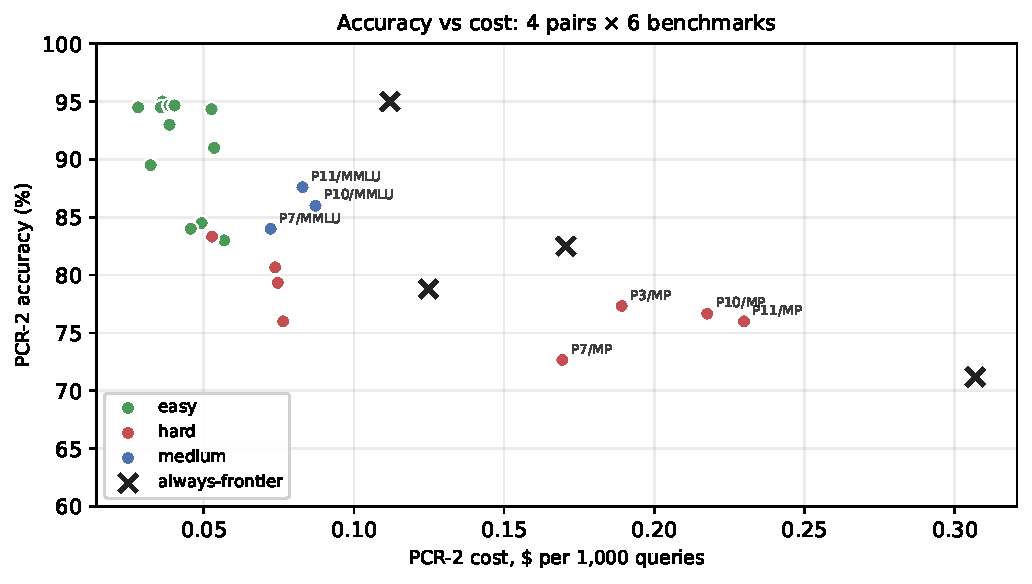
\includegraphics[width=\columnwidth]{fig_acc_cost}
\caption{PCR-2 accuracy vs.\ cost per 1{,}000 queries for the 4 complete pairs
$\times$ 6 benchmarks, coloured by difficulty tier. $\times$ = Always-Frontier
(gpt-oss-120B run solo) at its own cost and accuracy. Easy points are up-left of
the frontier; the MMLU and MMLU-Pro points sit above it.}
\label{fig:tradeoff}
\end{figure}

\begin{table}[!t]
\caption{Measured cost and latency for the 4 complete pairs (per-call
instrumentation; representative rows ordered by cost cut). Cost = list-price
tokens; runs were free-tier. AF = always-frontier.}
\label{tab:cost}
\renewcommand{\arraystretch}{1.15}
\begin{tabular}{l c c c c c}
\toprule
\textbf{Pair / bench} & \textbf{Esc.} & \textbf{\$/1k PCR} & \textbf{\$/1k AF} & \textbf{cut} & \textbf{lat.} \\
\midrule
Pair 7 / OpenBookQA & 5.0\% & 0.028 & 0.100 & 72\% & 0.49\,s \\
Pair 7 / CommonsenseQA & 8.5\% & 0.032 & 0.104 & 69\% & 0.55\,s \\
Pair 7 / ARC & 4.0\% & 0.036 & 0.108 & 66\% & 0.40\,s \\
Pair 10 / OpenBookQA & 9.0\% & 0.036 & 0.092 & 61\% & 4.31\,s \\
Pair 7 / TruthfulQA & 11.3\% & 0.053 & 0.130 & 59\% & 0.38\,s \\
Pair 11 / MMLU & 18.4\% & 0.083 & 0.172 & 52\% & 1.27\,s \\
Pair 10 / MMLU & 21.2\% & 0.087 & 0.170 & 49\% & 1.94\,s \\
Pair 3 / MMLU-Pro & 24.0\% & 0.189 & 0.349 & 46\% & 1.55\,s \\
Pair 7 / MMLU-Pro & 28.0\% & 0.169 & 0.287 & 41\% & 0.63\,s \\
Pair 10 / TruthfulQA & 30.0\% & 0.075 & 0.122 & 39\% & 1.03\,s \\
Pair 11 / MMLU-Pro & 50.0\% & 0.230 & 0.294 & 22\% & 3.06\,s \\
\bottomrule
\end{tabular}
\end{table}

Latency is set by the slowest cheap model, not the policy: Pair~7 (both Qwen3
27B on Groq) runs PCR-2 at \textbf{0.4--0.6\,s on every benchmark}, whereas
Pairs~10/11 (which pair \texttt{gpt-oss-20B} with Qwen) run at \textbf{0.9--5.7\,s}
--- \texttt{gpt-oss-20B}'s reasoning prelude, not the extra model or the
provider, is the cost. For a latency-sensitive deployment the cheap pair should
be two \textit{non-reasoning} small models on the same fast provider.

\subsection{Finding 4: PCR-3 does not help}
A third cheap model (all-Groq trio, $N=120$/benchmark) breaks nearly every tie
(a 2-of-3 majority forms 84--100\% of the time), collapsing escalation---but
buys \textbf{no accuracy and no safety} (Table~\ref{tab:pcr3}). C-Hall is
flat-to-worse on every benchmark: the items that stop escalating are added to
the trusted set without being any cleaner. PCR-3 trades one frontier call for
one extra cheap call per query---net-negative on easy/medium, roughly
break-even on hard. \textbf{Binary-agreement PCR-2 with a matched pair remains
the right design.}

\begin{table}[!t]
\caption{PCR-3 (gpt-oss-20b + qwen3.6-27b + qwen3.8-27b, majority vote) vs.\
PCR-2 (Pair 7, the same two Qwen models). $N=120$.}
\label{tab:pcr3}
\renewcommand{\arraystretch}{1.2}
\begin{tabular}{l c c c c}
\toprule
\textbf{Benchmark} & \textbf{Policy} & \textbf{Esc.} & \textbf{C-Hall} & \textbf{Overall acc.} \\
\midrule
\multirow{2}{*}{ARC} & PCR-2 & 4.0\% & 2.6\% & 95.0\% \\
 & PCR-3 & \textbf{0\%} & 5.0\% & 95.0\% \\
\multirow{2}{*}{TruthfulQA} & PCR-2 & 11.3\% & 14.3\% & 83.3\% \\
 & PCR-3 & \textbf{1\%} & 18.5\% & 81.7\% \\
\multirow{2}{*}{MMLU-Pro} & PCR-2 & 28.0\% & 25.9\% & 72.7\% \\
 & PCR-3 & \textbf{16\%} & 28.7\% & 73.3\% \\
\bottomrule
\end{tabular}
\end{table}

\subsection{Finding 5: Model family --- agreement premium on hard questions;
a suggestive C-Hall premium there too}
On the balanced 4-pair design (2 within, 2 cross, all 6 benchmarks, shared
frontier and provider), bootstrap 95\% CIs on the within-minus-cross gap
(Table~\ref{tab:family}) split cleanly by difficulty.
\textbf{Agreement.} On the easy benchmarks (ARC, OpenBookQA) both conditions
agree $\sim$90--96\% and the gap is null. On the hard/adversarial benchmarks the
within-family pairs agree far more: CommonsenseQA $+9.0$, TruthfulQA $+14.0$,
MMLU-Pro $+21.7$\,pp, every CI excluding 0. MMLU \textit{reverses}
($-7.2$\,pp, CI $[-12.2,-2.0]$) because Pair~3's safety-tuned Cheap~B refuses or
hedges on many items, cutting that pair's agreement to 58\%.
\textbf{Coordinated hallucination} follows the same shape, one step weaker: null
on ARC, OpenBookQA, MMLU and CommonsenseQA (CIs span 0), but positive on the two
hardest benchmarks --- \textbf{TruthfulQA $+6.6$\,pp, CI $[+0.3,+12.8]$}
(excludes 0) and \textbf{MMLU-Pro $+7.2$\,pp, CI $[-0.3,+14.9]$} (right at the
boundary). The pair-level balanced gap is $+3.4$\,pp.
\textbf{Read conservatively: shared lineage buys a large agreement premium on
hard questions, and \textit{plausibly} a coordinated-hallucination premium there
too --- but with only two pairs per condition the C-Hall signal is a hypothesis
for a powered replication, not a settled result.} On easy and medium questions
neither effect is present; what dominates C-Hall everywhere is benchmark
difficulty (Finding 1). Note also that on TruthfulQA the capability gap runs
\textit{against} this result --- the cross-family pairs are the mismatched ones
there (10--12.6\,pp, Table~\ref{tab:solo}), which should inflate \textit{their}
C-Hall, yet they show the lower rate.

\begin{table}[!t]
\caption{Within-family minus cross-family gap on the balanced 4-pair design.}
\label{tab:family}
\renewcommand{\arraystretch}{1.15}
\begin{tabular}{l r r r l}
\toprule
\textbf{Benchmark} & \textbf{within} & \textbf{cross} & \textbf{gap} & \textbf{95\% CI} \\
\midrule
\multicolumn{5}{l}{\textit{Agreement rate}} \\
ARC & 95.4 & 94.0 & $+1.4$ & $[-1.8,+4.7]$ \\
OpenBookQA & 92.2 & 89.5 & $+2.7$ & $[-1.3,+6.8]$ \\
MMLU & 73.0 & 80.2 & $-7.2$ & $[-12.2,-2.0]^\ast$ \\
CommonsenseQA & 90.8 & 81.8 & $+9.0$ & $[+4.2,+13.5]^\ast$ \\
TruthfulQA & 84.7 & 70.7 & $+14.0$ & $[+7.7,+20.3]^\ast$ \\
MMLU-Pro & 74.0 & 52.3 & $+21.7$ & $[+14.0,+29.3]^\ast$ \\
\midrule
\multicolumn{5}{l}{\textit{Coordinated hallucination}} \\
ARC & 3.4 & 2.8 & $+0.5$ & $[-2.1,+2.9]$ \\
OpenBookQA & 3.3 & 2.2 & $+1.0$ & $[-1.3,+3.4]$ \\
MMLU & 10.1 & 10.0 & $+0.2$ & $[-4.0,+4.3]$ \\
CommonsenseQA & 11.3 & 8.6 & $+2.7$ & $[-1.8,+7.3]$ \\
TruthfulQA & 16.9 & 10.4 & $+6.6$ & $[+0.3,+12.8]^\ast$ \\
MMLU-Pro & 22.5 & 15.3 & $+7.2$ & $[-0.3,+14.9]$ \\
\bottomrule
\multicolumn{5}{p{8.4cm}}{\footnotesize $^\ast$CI excludes 0. Question-level bootstrap, 10{,}000 iterations, over the 4 complete pairs (within = Pairs 3, 7; cross = Pairs 10, 11). Two pairs per condition --- treat the C-Hall column as suggestive.}
\end{tabular}
\end{table}


\subsection{Finding 6: Capability matching is what makes a pair usable}
\label{sec:capmatch}
Binary agreement is only a quality signal when both cheap models are
\textit{comparably} capable. If one is materially weaker, its errors dominate the
agreed set: on items the weak model cannot do, it frequently lands on the same
plausible-but-wrong distractor the stronger model would only occasionally pick,
and the pair ``agrees'' on a wrong answer. The resulting C-Hall measures a
\textbf{skill gap, not shared blind spots} --- it is not evidence about lineage,
and a study that mixes matched and mismatched pairs will read the former as the
latter.

We therefore adopted a $\pm3$\,pp solo-accuracy matching bar as an \textit{a
priori} screening criterion (\S\ref{sec:inclusion}); it is the single largest
reason candidate pairs were dropped. Within the four pairs retained, the bar
holds on ARC, MMLU and MMLU-Pro, and the one place it does not --- TruthfulQA,
where the cross-family pairs carry 10--12.6\,pp gaps (Table~\ref{tab:solo}) ---
biases against rather than toward our family conclusion (Finding~5).

The practical corollary for practitioners is blunt: \textbf{do not build a PCR
pair from two models of visibly different strength}, and in particular not from
two sizes of the same model series, which are mismatched by construction. Verify
the gap on the target distribution before deploying, not after.

\subsection{Per-pair, per-benchmark grid}
All results use the \textbf{four pairs with a complete six-benchmark
grid}: two within-family (Pair~3, gpt-oss + gpt-oss-safeguard; Pair~7, Qwen3.6 +
Qwen3.8) and two cross-family (Pair~10, gpt-oss-20B + Qwen3.6; Pair~11,
gpt-oss-20B + Qwen3.8). All four hold the frontier constant (gpt-oss-120B) and
run on one provider, so provider and frontier are controlled and only lineage
varies (\S\ref{sec:inclusion}).

Table~\ref{tab:percell} gives the $4\times6$ grid for the two quantities that
carry the paper's argument. Two patterns: (i) C-Hall tracks benchmark difficulty
monotonically for every pair ($\sim$2--5\% ARC/OpenBookQA, $\sim$7--16\%
MMLU/CommonsenseQA, $\sim$10--20\% TruthfulQA, $\sim$13--26\% MMLU-Pro); (ii) the
within-family pairs sit at the high end of agreement on the hard/adversarial
benchmarks but \textit{not} on MMLU, where Pair~3's safety-tuned Cheap~B model
refuses or hedges, cutting agreement to 58\%.

\begin{table}[!t]
\caption{The consistent $4\times6$ grid, PCR-2. \textbf{Top:}
coordinated-hallucination rate (\%) on agreed questions. \textbf{Bottom:}
agreement rate (\%). ``(w)'' = within-family. Frontier = gpt-oss-120B for all
four; all on Groq.}
\label{tab:percell}
\renewcommand{\arraystretch}{1.2}
\footnotesize
\setlength{\tabcolsep}{5pt}
\begin{tabular}{l c c c c c c}
\toprule
\multicolumn{7}{c}{\textit{Coordinated hallucination (\%)}} \\
\midrule
\textbf{Pair} & \textbf{ARC} & \textbf{MMLU} & \textbf{M-Pro} & \textbf{TQA} & \textbf{OBQA} & \textbf{CSQA} \\
\midrule
3\,{\footnotesize(w)} & 3.9 & 8.3 & 19.3 & 19.8 & 4.5 & 15.6 \\
7\,{\footnotesize(w)} & 2.6 & 11.3 & 25.9 & 14.3 & 2.1 & 7.1 \\
10 & 2.8 & 9.6 & 17.1 & 9.5 & 1.6 & 7.4 \\
11 & 2.9 & 10.3 & 13.3 & 11.2 & 2.8 & 9.7 \\
\midrule
\multicolumn{7}{c}{\textit{Agreement rate (\%)}} \\
\midrule
\textbf{Pair} & \textbf{ARC} & \textbf{MMLU} & \textbf{M-Pro} & \textbf{TQA} & \textbf{OBQA} & \textbf{CSQA} \\
\midrule
3\,{\footnotesize(w)} & 95 & 58 & 76 & 81 & 90 & 90 \\
7\,{\footnotesize(w)} & 96 & 88 & 72 & 89 & 95 & 92 \\
10 & 95 & 79 & 55 & 70 & 91 & 81 \\
11 & 93 & 82 & 50 & 71 & 88 & 82 \\
\bottomrule
\end{tabular}
\end{table}

\subsection{When the second cheap model earns its call}
\label{sec:earns}
Table~\ref{tab:netgain} decomposes PCR-2 against the strongest single cheap model
(the policy a practitioner would fall back to) and shows the escalation rate that
drives its cost. Three things stand out.

\textbf{The value is concentrated on the hard tier.} PCR-2 beats Best-Cheap by
$+10$ to $+11$\,pp on MMLU-Pro for Pairs~7/10/11, and by $+15.6$\,pp on MMLU for
Pair~3 (whose weak safety-tuned Cheap~B drags Best-Cheap down while consensus
still filters well). On ARC the gap is $\pm1$\,pp.

\textbf{On the ``easy'' knowledge benchmarks PCR-2 can lose.} On OpenBookQA all
four pairs come in $1$--$2.5$\,pp \textit{below} Best-Cheap, and the cross-family
pairs are $2$--$4$\,pp below on CommonsenseQA. When cheap models are already near
ceiling, the $\sim$10--20\% of queries that escalate flip about as many correct
answers to wrong as they rescue --- 9 of the 24 cells are net negative, eight of
them on the easy tier (the ninth is Pair~10 on TruthfulQA). \textbf{PCR-2 is a middle-of-the-difficulty-range tool}: skip it where
a single cheap model already clears $\sim$92\%.

\textbf{Escalation rate is a free difficulty gauge.} It rises monotonically with
benchmark difficulty for every pair (4--7\% ARC $\to$ 12--42\% MMLU $\to$
24--50\% MMLU-Pro) without any labels or training --- the router's own
disagreement signal is an unsupervised estimate of query hardness that a
deployment can log and act on.

\begin{table}[!t]
\caption{\textbf{Top:} PCR-2 accuracy minus the stronger cheap model's solo
accuracy (pp) --- positive = the second model plus escalation helps.
\textbf{Bottom:} escalation rate (\%). ``(w)'' = within-family.}
\label{tab:netgain}
\renewcommand{\arraystretch}{1.2}
\footnotesize
\setlength{\tabcolsep}{5pt}
\begin{tabular}{l c c c c c c}
\toprule
\multicolumn{7}{c}{\textit{PCR-2 $-$ Best-Cheap (pp)}} \\
\midrule
\textbf{Pair} & \textbf{ARC} & \textbf{MMLU} & \textbf{M-Pro} & \textbf{TQA} & \textbf{OBQA} & \textbf{CSQA} \\
\midrule
3\,{\footnotesize(w)} & $+0.7$ & $+15.6$ & $+3.3$ & $+4.7$ & $-1.0$ & $+3.0$ \\
7\,{\footnotesize(w)} & $-0.5$ & $+0.8$ & $+10.7$ & $+2.0$ & $-2.0$ & $0.0$ \\
10 & $-0.7$ & $+3.2$ & $+11.3$ & $-2.7$ & $-2.5$ & $-4.0$ \\
11 & $+0.7$ & $+4.4$ & $+10.0$ & $+1.3$ & $-1.5$ & $-2.0$ \\
\midrule
\multicolumn{7}{c}{\textit{Escalation rate (\%)}} \\
\midrule
\textbf{Pair} & \textbf{ARC} & \textbf{MMLU} & \textbf{M-Pro} & \textbf{TQA} & \textbf{OBQA} & \textbf{CSQA} \\
\midrule
3\,{\footnotesize(w)} & 5 & 42 & 24 & 19 & 10 & 10 \\
7\,{\footnotesize(w)} & 4 & 12 & 28 & 11 & 5 & 8 \\
10 & 5 & 21 & 45 & 30 & 9 & 19 \\
11 & 7 & 18 & 50 & 29 & 12 & 18 \\
\bottomrule
\end{tabular}
\end{table}

\subsection{Practitioner recommendations}
The four complete pairs also settle the practitioner question directly. The
recommended default, \textbf{Pair~7 (Qwen3.6-27B + Qwen3.8-27B $\to$
gpt-oss-120B, all Groq)}, holds 90--95\% on easy, 84\% on MMLU (vs.\ 82.5\% for
always-frontier) and 73--83\% on the hard tier, at 0.4--0.6\,s and 41--72\%
below always-frontier cost. The cross-family alternative, \textbf{Pairs~10/11
(gpt-oss-20B + Qwen)}, matches it on accuracy --- in fact edges ahead on MMLU
(86--88\%) and the hard tier (76--78\%) because the two developers' errors are
less correlated --- but runs 2--10$\times$ slower and escalates more (Table~%
\ref{tab:netgain}). Choose Pair~7 when latency dominates, Pair~10/11 when the
workload leans hard and independence matters.

\begin{table}[!t]
\caption{Recommended configuration by goal (free-tier, 2026).}
\label{tab:recs}
\renewcommand{\arraystretch}{1.25}
\begin{tabular}{p{2.4cm} p{2.7cm} p{2.7cm}}
\toprule
\textbf{Goal} & \textbf{Use} & \textbf{Why} \\
\midrule
High-volume, mostly easy/medium; minimise cost + latency
& PCR-2: qwen3.6-27b + qwen3.8-27b $\to$ gpt-oss-120b (all Groq)
& $\approx$Best-Cheap / Always-Frontier accuracy; 41--72\% cheaper; 0.4--0.6\,s;
4--12\% escalation outside MMLU-Pro (28\% there); no truncation. \\
Hard-leaning workload; want error-independence
& PCR-2: gpt-oss-20b + qwen3.8-27b $\to$ gpt-oss-120b (Pair~11, all Groq)
& Different developers $\Rightarrow$ less-correlated errors; +4\,pp on MMLU,
+10\,pp on MMLU-Pro over Best-Cheap. Cost: 1--3\,s, higher escalation. \\
Easy benchmarks where a cheap model already clears $\sim$92\%
& Skip PCR; use the stronger cheap model alone
& On OpenBookQA/CommonsenseQA PCR-2 is 1--4\,pp \textit{below} Best-Cheap
(Table~\ref{tab:netgain}) --- escalation flips as many right as it fixes. \\
Hard / adversarial queries
& Do not use PCR consensus as a trust signal; route to frontier or gate by
difficulty
& Agreement is 10--26\% wrong there; PCR-2 gains +3--11\,pp on MMLU-Pro but
ships confident errors and is only 22--46\% cheaper. \\
Research: settle the family question
& $\geq$3 capability-matched pairs / condition, $N\!\approx\!1000$ on MMLU-Pro
& Only MMLU/MMLU-Pro pools are large enough; each pair must clear the
$\pm3$\,pp bar. \\
\bottomrule
\end{tabular}
\end{table}

%===========================================================
\section{Conclusion}
%===========================================================
Parallel Consensus Routing uses inter-model binary agreement as a training-free,
black-box quality oracle and is the first routing approach to formalize the
speculative-decoding analogy at the response level. On a balanced four-pair
design spanning a complete six-benchmark grid --- every pair evaluated on every
benchmark, frontier and provider held constant --- with an eight-policy
ablation, we establish:
(1) coordinated hallucination scales monotonically with question difficulty
($\approx$3\% to $\approx$19\% mean, up to 26\% for the within-family pair), not
with task type; (2) a capability-matched cheap pair
with PCR-2 matches always-frontier accuracy on easy/medium queries at 40--70\%
lower cost, but is unsafe on hard queries where 12--26\% of trusted answers are
wrong; (3) shared model lineage buys a large agreement premium on
hard/adversarial benchmarks and, suggestively, a coordinated-hallucination
premium there too (TruthfulQA $+6.6$\,pp) --- underpowered at two pairs per
condition, so a hypothesis for replication; capability matching, not lineage, is
what makes a pair usable; (4) a third cheap model breaks ties but adds no
accuracy or safety; (5) on free-tier APIs, two of \{gpt-oss-20B, Qwen3.6-27B,
Qwen3.8-27B\} on a low-latency provider is the recommended default.
The practical consequence is that a PCR deployment needs a
	extit{difficulty}-calibrated trust threshold rather than a task-type rule: the
router's own escalation rate supplies that difficulty estimate for free.

\subsection*{Limitations}
Pilot-scale $N$ (150--300 per cell) gives per-benchmark C-Hall CIs of
$\pm3$--14\,pp, and the family comparison rests on two pairs per condition --- the
hard-tier C-Hall premium (Finding~5) needs a powered replication before it can be
claimed. Restricting to pairs with complete coverage buys internal consistency at
the cost of breadth: all four pairs are served by one provider and share one
frontier, so \textbf{provider and frontier are held constant but also
unvaried} --- we cannot say whether the findings transfer to a different
frontier or a slower serving stack, and a capability-matched within-family pair
on a second provider remains the key missing replicate. On TruthfulQA the two
cross-family pairs exceed the $\pm3$\,pp matching bar (10--12.6\,pp,
Table~\ref{tab:solo}); the bias runs against Finding~5 rather than for it, but the
cell is not cleanly matched. Pair~3's Cheap~B is a safety-tuned model that refuses
or hedges on $\sim$40\% of MMLU items, halving its agreement and inflating
escalation without inflating accuracy --- \textbf{safety-tuned models are poor PCR
cheap models}, and it was retained only because it is the one available
same-lineage partner for gpt-oss-20B. Cosine similarity between raw responses is
unavailable in this run (a library incompatibility), so we report binary letter
agreement only. Always-Frontier is a single model (gpt-oss-120b). All runs used
free-tier APIs; paid-tier cost profiles differ.

\subsection*{Future Work}
\label{sec:futurework}
A statistically powered family study ($\approx$1000 MMLU-Pro questions
$\times\geq$3 matched pairs per condition, on at least two providers) would let
the hard-tier C-Hall premium be \textit{claimed} rather than merely suggested.
The 3--5\,pp Oracle-2-cheap gap motivates a lightweight learned selector beyond
binary agreement. Extending the grid to a \textbf{numeric-answer benchmark}
requires first disentangling answer extraction from the token budget: a truncated
multi-step solution yields an intermediate value that a last-number parser scores
as a disagreement, so apparent C-Hall on such benchmarks is budget-sensitive and
must be calibrated before it can be compared against the multiple-choice grid.
Online difficulty threshold learning \cite{schroeder2025vcache} would remove the
calibration corpus. Extending PCR to open-ended generation needs a semantic
agreement criterion; applying it to retrieval-augmented generation
\cite{lewis2020rag}, where grounded facts may still be co-hallucinated, is a
high-value target.

%===========================================================
\balance
\bibliographystyle{IEEEtran}
\begin{thebibliography}{99}

\bibitem{bommasani2021}
R. Bommasani, D.~A. Hudson, et al., ``On the opportunities and risks of foundation models,'' arXiv:2108.07258, 2021.

\bibitem{ong2024routellm}
I. Ong, A. Almahairi, V. Wu, W.-L. Chiang, T. Wu, J.~E. Gonzalez, M.~W. Kadous, and I. Stoica, ``RouteLLM: Learning to route LLMs with preference data,'' arXiv:2406.18665, 2024.

\bibitem{ding2024hybrid}
D. Ding, A. Mallick, C. Wang, R. Sim, S. Mukherjee, V. Ruhle, L.~V.~S. Lakshmanan, and A.~H. Awadallah, ``Hybrid LLM: Cost-efficient and quality-aware query routing,'' in \textit{Proc.\ ICLR}, arXiv:2404.14618, 2024.

\bibitem{chen2023frugalgpt}
L. Chen, M. Zaharia, and J. Zou, ``FrugalGPT: How to use large language models while reducing cost and improving performance,'' \textit{TMLR}, arXiv:2305.05176, 2023.

\bibitem{leviathan2023}
Y. Leviathan, M. Kalman, and Y. Matias, ``Fast inference from transformers via speculative decoding,'' in \textit{Proc.\ ICML}, PMLR 202, 2023.

\bibitem{chen2023speculative}
C. Chen, S. Borgeaud, G. Irving, J.-B. Lespiau, L. Sifre, and J. Jumper, ``Accelerating large language model decoding with speculative sampling,'' arXiv:2302.01318, 2023.

\bibitem{aggarwal2024automix}
P. Aggarwal, A. Madaan, A. Anand, et al., ``AutoMix: Automatically mixing language models,'' in \textit{Proc.\ ACL}, arXiv:2310.12963, 2024.

\bibitem{du2023multiagent}
Y. Du, S. Li, A. Torralba, J.~B. Tenenbaum, and I. Mordatch, ``Improving factuality and reasoning in language models through multiagent debate,'' in \textit{Proc.\ ICML}, arXiv:2305.14325, 2024.

\bibitem{jiang2023llmblender}
D. Jiang, X. Ren, and B.~Y. Lin, ``LLM-Blender: Ensembling large language models with pairwise ranking and generative fusion,'' in \textit{Proc.\ ACL}, pp.\ 14165--14178, 2023.

\bibitem{wang2023selfconsistency}
X. Wang, J. Wei, D. Schuurmans, Q. Le, E. Chi, S. Narang, A. Chowdhery, and D. Zhou, ``Self-consistency improves chain of thought reasoning in language models,'' in \textit{Proc.\ ICLR}, arXiv:2203.11171, 2023.

\bibitem{schroeder2025vcache}
L.~G. Schroeder, A. Desai, A. Cuadron, et al., ``vCache: Verified semantic prompt caching,'' arXiv:2502.03771, 2025.

\bibitem{manakul2023selfcheckgpt}
P. Manakul, A. Liusie, and M.~J.~F. Gales, ``SelfCheckGPT: Zero-resource black-box hallucination detection for generative large language models,'' in \textit{Proc.\ EMNLP}, pp.\ 9004--9017, 2023.

\bibitem{kadavath2022}
S. Kadavath, T. Conerly, A. Askell, et al., ``Language models (mostly) know what they know,'' arXiv:2207.05221, 2022.

\bibitem{hendrycks2020mmlu}
D. Hendrycks, C. Burns, S. Basart, A. Zou, M. Mazeika, D. Song, and J. Steinhardt, ``Measuring massive multitask language understanding,'' arXiv:2009.03300, 2020.

\bibitem{cobbe2021gsm8k}
K. Cobbe, V. Kosaraju, M. Bavarian, et al., ``Training verifiers to solve math word problems,'' arXiv:2110.14168, 2021.

\bibitem{clark2018arc}
P. Clark, I. Cowhey, O. Etzioni, T. Khot, A. Sabharwal, C. Schoenick, and O. Tafjord, ``Think you have solved question answering? Try ARC, the AI2 Reasoning Challenge,'' arXiv:1803.05457, 2018.

\bibitem{lin2022truthfulqa}
S. Lin, J. Hilton, and O. Evans, ``TruthfulQA: Measuring how models mimic human falsehoods,'' in \textit{Proc.\ ACL}, arXiv:2109.07958, 2022.

\bibitem{wang2024mmlupro}
Y. Wang, X. Ma, G. Zhang, et al., ``MMLU-Pro: A more robust and challenging multi-task language understanding benchmark,'' in \textit{Proc.\ NeurIPS Datasets and Benchmarks}, arXiv:2406.01574, 2024.

\bibitem{mihaylov2018openbookqa}
T. Mihaylov, P. Clark, T. Khot, and A. Sabharwal, ``Can a suit of armor conduct electricity? A new dataset for open book question answering,'' in \textit{Proc.\ EMNLP}, arXiv:1809.02789, 2018.

\bibitem{talmor2019csqa}
A. Talmor, J. Herzig, N. Lourie, and J. Berant, ``CommonsenseQA: A question answering challenge targeting commonsense knowledge,'' in \textit{Proc.\ NAACL-HLT}, arXiv:1811.00937, 2019.

\bibitem{hu2024routerbench}
Q.~J. Hu, J. Bieker, X. Li, et al., ``RouterBench: A benchmark for multi-LLM routing system,'' arXiv:2403.12031, 2024.

\bibitem{reimers2019sentencebert}
N. Reimers and I. Gurevych, ``Sentence-BERT: Sentence embeddings using siamese BERT-networks,'' in \textit{Proc.\ EMNLP-IJCNLP}, pp.\ 3982--3992, 2019.

\bibitem{wei2022cot}
J. Wei, X. Wang, D. Schuurmans, et al., ``Chain-of-thought prompting elicits reasoning in large language models,'' in \textit{Proc.\ NeurIPS}, arXiv:2201.11903, 2022.

\bibitem{sakota2024forc}
M. Sakota, M. Peyrard, and H. Schutze, ``FORC: Fine-grained orchestration for LLM routing with contrastive learning,'' arXiv:2402.09997, 2024.

\bibitem{feng2024graphrouter}
T. Feng, Y. Shen, and J. You, ``GraphRouter: A graph-based router for LLM selections,'' arXiv:2410.03834, 2024.

\bibitem{chan2023chateval}
C.-M. Chan, W. Chen, Y. Su, et al., ``ChatEval: Towards better LLM-based evaluators through multi-agent debate,'' arXiv:2308.07201, 2023.

\bibitem{lewis2020rag}
P. Lewis, E. Perez, A. Piktus, et al., ``Retrieval-augmented generation for knowledge-intensive NLP tasks,'' in \textit{Proc.\ NeurIPS}, arXiv:2005.11401, 2020.

\end{thebibliography}

\end{document}
